\begin{frame}{Οδομετρία μέσω lidar (real)}

%\begin{figure}
  %\definecolor{plicp}{rgb}{0.00000   0.44700   0.74100}
\definecolor{ndt}{rgb}{0.85000   0.32500   0.09800}
\definecolor{fgi}{rgb}{0.9290 0.6940 0.1250}
\definecolor{fvg}{rgb}{0.4940 0.1840 0.5560}
\definecolor{fmt}{rgb}{1.00000   0.00000   1.00000}
\definecolor{gg}{RGB}{156 156 156}

% GNUPLOT: LaTeX picture with Postscript
\begingroup
  \makeatletter
  \providecommand\color[2][]{%
    \GenericError{(gnuplot) \space\space\space\@spaces}{%
      Package color not loaded in conjunction with
      terminal option `colourtext'%
    }{See the gnuplot documentation for explanation.%
    }{Either use 'blacktext' in gnuplot or load the package
      color.sty in LaTeX.}%
    \renewcommand\color[2][]{}%
  }%
  \providecommand\includegraphics[2][]{%
    \GenericError{(gnuplot) \space\space\space\@spaces}{%
      Package graphicx or graphics not loaded%
    }{See the gnuplot documentation for explanation.%
    }{The gnuplot epslatex terminal needs graphicx.sty or graphics.sty.}%
    \renewcommand\includegraphics[2][]{}%
  }%
  \providecommand\rotatebox[2]{#2}%
  \@ifundefined{ifGPcolor}{%
    \newif\ifGPcolor
    \GPcolorfalse
  }{}%
  \@ifundefined{ifGPblacktext}{%
    \newif\ifGPblacktext
    \GPblacktexttrue
  }{}%
  % define a \g@addto@macro without @ in the name:
  \let\gplgaddtomacro\g@addto@macro
  % define empty templates for all commands taking text:
  \gdef\gplfronttext{}%
  \gdef\gplfronttext{}%
  \makeatother
  \ifGPblacktext
    % no textcolor at all
    \def\colorrgb#1{}%
    \def\colorgray#1{}%
  \else
    % gray or color?
    \ifGPcolor
      \def\colorrgb#1{\color[rgb]{#1}}%
      \def\colorgray#1{\color[gray]{#1}}%
      \expandafter\def\csname LTw\endcsname{\color{white}}%
      \expandafter\def\csname LTb\endcsname{\color{black}}%
      \expandafter\def\csname LTa\endcsname{\color{black}}%
      \expandafter\def\csname LT0\endcsname{\color[rgb]{1,0,0}}%
      \expandafter\def\csname LT1\endcsname{\color[rgb]{0,1,0}}%
      \expandafter\def\csname LT2\endcsname{\color[rgb]{0,0,1}}%
      \expandafter\def\csname LT3\endcsname{\color[rgb]{1,0,1}}%
      \expandafter\def\csname LT4\endcsname{\color[rgb]{0,1,1}}%
      \expandafter\def\csname LT5\endcsname{\color[rgb]{1,1,0}}%
      \expandafter\def\csname LT6\endcsname{\color[rgb]{0,0,0}}%
      \expandafter\def\csname LT7\endcsname{\color[rgb]{1,0.3,0}}%
      \expandafter\def\csname LT8\endcsname{\color[rgb]{0.5,0.5,0.5}}%
    \else
      % gray
      \def\colorrgb#1{\color{black}}%
      \def\colorgray#1{\color[gray]{#1}}%
      \expandafter\def\csname LTw\endcsname{\color{white}}%
      \expandafter\def\csname LTb\endcsname{\color{black}}%
      \expandafter\def\csname LTa\endcsname{\color{black}}%
      \expandafter\def\csname LT0\endcsname{\color{black}}%
      \expandafter\def\csname LT1\endcsname{\color{black}}%
      \expandafter\def\csname LT2\endcsname{\color{black}}%
      \expandafter\def\csname LT3\endcsname{\color{black}}%
      \expandafter\def\csname LT4\endcsname{\color{black}}%
      \expandafter\def\csname LT5\endcsname{\color{black}}%
      \expandafter\def\csname LT6\endcsname{\color{black}}%
      \expandafter\def\csname LT7\endcsname{\color{black}}%
      \expandafter\def\csname LT8\endcsname{\color{black}}%
    \fi
  \fi
    \setlength{\unitlength}{0.0500bp}%
    \ifx\gptboxheight\undefined%
      \newlength{\gptboxheight}%
      \newlength{\gptboxwidth}%
      \newsavebox{\gptboxtext}%
    \fi%
    \setlength{\fboxrule}{0.5pt}%
    \setlength{\fboxsep}{1pt}%
\begin{picture}(8000.00,4000.00)%
    \gplgaddtomacro\gplfronttext{%
      \put(1000,3900){\makebox(0,0){\strut{}{\color{plicp}{\rule[0.6mm]{0.5cm}{0.5mm}}} PLICP}}
      \put(2500,3900){\makebox(0,0){\strut{}{\color{ndt}{\rule[0.6mm]{0.5cm}{0.5mm}}} NDT}}
      \put(4000,3900){\makebox(0,0){\strut{}{\color{fgi}{\rule[0.6mm]{0.5cm}{0.5mm}}} GICP}}
      \put(5500,3900){\makebox(0,0){\strut{}{\color{fvg}{\rule[0.6mm]{0.5cm}{0.5mm}}} VGICP}}
      \put(7000,3900){\makebox(0,0){\strut{}{\color{fmt}{\rule[0.6mm]{0.5cm}{0.5mm}}} \texttt{fsm}}}
    }%
    \gplgaddtomacro\gplfronttext{%
      \colorrgb{0.15,0.15,0.15}%
      \put(953,3206){\makebox(0,0)[r]{\strut{}$21.0$}}%
      \colorrgb{0.15,0.15,0.15}%
      \put(953,2466){\makebox(0,0)[r]{\strut{}$19.0$}}%
      \colorrgb{0.15,0.15,0.15}%
      \put(953,1726){\makebox(0,0)[r]{\strut{}$17.0$}}%
      \colorrgb{0.15,0.15,0.15}%
      \put(953,986){\makebox(0,0)[r]{\strut{}$15.0$}}%
      \colorrgb{0.15,0.15,0.15}%
      \put(1455,3326){\makebox(0,0){\strut{}$12.0$}}%
      \colorrgb{0.15,0.15,0.15}%
      \put(2935,3326){\makebox(0,0){\strut{}$16.0$}}%
      \colorrgb{0.15,0.15,0.15}%
      \put(4416,3326){\makebox(0,0){\strut{}$20.0$}}%
      \colorrgb{0.15,0.15,0.15}%
      \put(5896,3326){\makebox(0,0){\strut{}$24.0$}}%
      \colorrgb{0.15,0.15,0.15}%
      \put(7376,3326){\makebox(0,0){\strut{}$28.0$}}%
    }%
    \put(0,0){\animategraphics[autoplay,loop]{0.5}{./figures/slides/ch7/odom/real/odom_test_ag10/odom_test_}{1}{10}}%
    \gplfronttext
  \end{picture}%
\endgroup

%\end{figure}

\begin{figure}\centering
  \begin{minipage}{0.5\textwidth}
    \centering
    \definecolor{plicp}{rgb}{0.00000   0.44700   0.74100}
\definecolor{ndt}{rgb}{0.85000   0.32500   0.09800}
\definecolor{fgi}{rgb}{0.9290 0.6940 0.1250}
\definecolor{fvg}{rgb}{0.4940 0.1840 0.5560}
\definecolor{fmt}{rgb}{1.00000   0.00000   1.00000}
\definecolor{gg}{RGB}{156 156 156}

% GNUPLOT: LaTeX picture with Postscript
\begingroup
  \makeatletter
  \providecommand\color[2][]{%
    \GenericError{(gnuplot) \space\space\space\@spaces}{%
      Package color not loaded in conjunction with
      terminal option `colourtext'%
    }{See the gnuplot documentation for explanation.%
    }{Either use 'blacktext' in gnuplot or load the package
      color.sty in LaTeX.}%
    \renewcommand\color[2][]{}%
  }%
  \providecommand\includegraphics[2][]{%
    \GenericError{(gnuplot) \space\space\space\@spaces}{%
      Package graphicx or graphics not loaded%
    }{See the gnuplot documentation for explanation.%
    }{The gnuplot epslatex terminal needs graphicx.sty or graphics.sty.}%
    \renewcommand\includegraphics[2][]{}%
  }%
  \providecommand\rotatebox[2]{#2}%
  \@ifundefined{ifGPcolor}{%
    \newif\ifGPcolor
    \GPcolorfalse
  }{}%
  \@ifundefined{ifGPblacktext}{%
    \newif\ifGPblacktext
    \GPblacktexttrue
  }{}%
  % define a \g@addto@macro without @ in the name:
  \let\gplgaddtomacro\g@addto@macro
  % define empty templates for all commands taking text:
  \gdef\gplfronttext{}%
  \gdef\gplfronttext{}%
  \makeatother
  \ifGPblacktext
    % no textcolor at all
    \def\colorrgb#1{}%
    \def\colorgray#1{}%
  \else
    % gray or color?
    \ifGPcolor
      \def\colorrgb#1{\color[rgb]{#1}}%
      \def\colorgray#1{\color[gray]{#1}}%
      \expandafter\def\csname LTw\endcsname{\color{white}}%
      \expandafter\def\csname LTb\endcsname{\color{black}}%
      \expandafter\def\csname LTa\endcsname{\color{black}}%
      \expandafter\def\csname LT0\endcsname{\color[rgb]{1,0,0}}%
      \expandafter\def\csname LT1\endcsname{\color[rgb]{0,1,0}}%
      \expandafter\def\csname LT2\endcsname{\color[rgb]{0,0,1}}%
      \expandafter\def\csname LT3\endcsname{\color[rgb]{1,0,1}}%
      \expandafter\def\csname LT4\endcsname{\color[rgb]{0,1,1}}%
      \expandafter\def\csname LT5\endcsname{\color[rgb]{1,1,0}}%
      \expandafter\def\csname LT6\endcsname{\color[rgb]{0,0,0}}%
      \expandafter\def\csname LT7\endcsname{\color[rgb]{1,0.3,0}}%
      \expandafter\def\csname LT8\endcsname{\color[rgb]{0.5,0.5,0.5}}%
    \else
      % gray
      \def\colorrgb#1{\color{black}}%
      \def\colorgray#1{\color[gray]{#1}}%
      \expandafter\def\csname LTw\endcsname{\color{white}}%
      \expandafter\def\csname LTb\endcsname{\color{black}}%
      \expandafter\def\csname LTa\endcsname{\color{black}}%
      \expandafter\def\csname LT0\endcsname{\color{black}}%
      \expandafter\def\csname LT1\endcsname{\color{black}}%
      \expandafter\def\csname LT2\endcsname{\color{black}}%
      \expandafter\def\csname LT3\endcsname{\color{black}}%
      \expandafter\def\csname LT4\endcsname{\color{black}}%
      \expandafter\def\csname LT5\endcsname{\color{black}}%
      \expandafter\def\csname LT6\endcsname{\color{black}}%
      \expandafter\def\csname LT7\endcsname{\color{black}}%
      \expandafter\def\csname LT8\endcsname{\color{black}}%
    \fi
  \fi
    \setlength{\unitlength}{0.0500bp}%
    \ifx\gptboxheight\undefined%
      \newlength{\gptboxheight}%
      \newlength{\gptboxwidth}%
      \newsavebox{\gptboxtext}%
    \fi%
    \setlength{\fboxrule}{0.5pt}%
    \setlength{\fboxsep}{1pt}%
\begin{picture}(8000.00,4000.00)%
    \gplgaddtomacro\gplfronttext{%
      \put( 500,3900){\makebox(0,0){\strut{}{\color{plicp}{\rule[0.6mm]{0.5cm}{0.5mm}}} PLICP}}
      \put(2000,3900){\makebox(0,0){\strut{}{\color{ndt}{\rule[0.6mm]{0.5cm}{0.5mm}}} NDT}}
      \put(3500,3900){\makebox(0,0){\strut{}{\color{fgi}{\rule[0.6mm]{0.5cm}{0.5mm}}} GICP}}
      \put(5000,3900){\makebox(0,0){\strut{}{\color{fvg}{\rule[0.6mm]{0.5cm}{0.5mm}}} VGICP}}
      \put(7000,3900){\makebox(0,0){\strut{}{\color{fmt}{\rule[0.6mm]{0.5cm}{0.5mm}}} \texttt{fsm}}}
    }%
    \gplgaddtomacro\gplfronttext{%
      \colorrgb{0.15,0.15,0.15}%
%      \put(953,3206){\makebox(0,0)[r]{\strut{}$21.0$}}%
      %\colorrgb{0.15,0.15,0.15}%
      %\put(953,2466){\makebox(0,0)[r]{\strut{}$19.0$}}%
      %\colorrgb{0.15,0.15,0.15}%
      %\put(953,1726){\makebox(0,0)[r]{\strut{}$17.0$}}%
      %\colorrgb{0.15,0.15,0.15}%
      %\put(953,986){\makebox(0,0)[r]{\strut{}$15.0$}}%
      \colorrgb{0.15,0.15,0.15}%
%      \put(1455,3326){\makebox(0,0){\strut{}$12.0$}}%
      %\colorrgb{0.15,0.15,0.15}%
      %\put(2935,3326){\makebox(0,0){\strut{}$16.0$}}%
      %\colorrgb{0.15,0.15,0.15}%
      %\put(4416,3326){\makebox(0,0){\strut{}$20.0$}}%
      %\colorrgb{0.15,0.15,0.15}%
      %\put(5896,3326){\makebox(0,0){\strut{}$24.0$}}%
      %\colorrgb{0.15,0.15,0.15}%
      %\put(7376,3326){\makebox(0,0){\strut{}$28.0$}}%
      \put( 85,  2760){\makebox(0,0){\strut{}\footnotesize $12.0$}}%
      \colorrgb{0.15,0.15,0.15}%
      \put(1076.6,2760){\makebox(0,0){\strut{}\footnotesize $16.0$}}%
      \colorrgb{0.15,0.15,0.15}%
      \put(2068.2,2760){\makebox(0,0){\strut{}\footnotesize $20.0$}}%
      \colorrgb{0.15,0.15,0.15}%
      \put(3059.8,2760){\makebox(0,0){\strut{}\footnotesize $24.0$}}%
      \colorrgb{0.15,0.15,0.15}%
      \put(4051.4,2760){\makebox(0,0){\strut{}\footnotesize $28.0$}}%
    }%
    \put(-900,500){\animategraphics[autoplay,loop,scale=0.67]{0.25}{./figures/slides/ch7/odom/real/odom_test_ag10/odom_test_}{1}{4}}%
    \gplfronttext
  \end{picture}%
\endgroup

  \end{minipage}\hfill
  \begin{minipage}{0.5\textwidth}
    \centering
    \definecolor{plicp}{rgb}{0.00000   0.44700   0.74100}
\definecolor{ndt}{rgb}{0.85000   0.32500   0.09800}
\definecolor{fgi}{rgb}{0.9290 0.6940 0.1250}
\definecolor{fvg}{rgb}{0.4940 0.1840 0.5560}
\definecolor{fmt}{rgb}{1.00000   0.00000   1.00000}
\definecolor{gg}{RGB}{156 156 156}

% GNUPLOT: LaTeX picture with Postscript
\begingroup
  \makeatletter
  \providecommand\color[2][]{%
    \GenericError{(gnuplot) \space\space\space\@spaces}{%
      Package color not loaded in conjunction with
      terminal option `colourtext'%
    }{See the gnuplot documentation for explanation.%
    }{Either use 'blacktext' in gnuplot or load the package
      color.sty in LaTeX.}%
    \renewcommand\color[2][]{}%
  }%
  \providecommand\includegraphics[2][]{%
    \GenericError{(gnuplot) \space\space\space\@spaces}{%
      Package graphicx or graphics not loaded%
    }{See the gnuplot documentation for explanation.%
    }{The gnuplot epslatex terminal needs graphicx.sty or graphics.sty.}%
    \renewcommand\includegraphics[2][]{}%
  }%
  \providecommand\rotatebox[2]{#2}%
  \@ifundefined{ifGPcolor}{%
    \newif\ifGPcolor
    \GPcolorfalse
  }{}%
  \@ifundefined{ifGPblacktext}{%
    \newif\ifGPblacktext
    \GPblacktexttrue
  }{}%
  % define a \g@addto@macro without @ in the name:
  \let\gplgaddtomacro\g@addto@macro
  % define empty templates for all commands taking text:
  \gdef\gplfronttext{}%
  \gdef\gplfronttext{}%
  \makeatother
  \ifGPblacktext
    % no textcolor at all
    \def\colorrgb#1{}%
    \def\colorgray#1{}%
  \else
    % gray or color?
    \ifGPcolor
      \def\colorrgb#1{\color[rgb]{#1}}%
      \def\colorgray#1{\color[gray]{#1}}%
      \expandafter\def\csname LTw\endcsname{\color{white}}%
      \expandafter\def\csname LTb\endcsname{\color{black}}%
      \expandafter\def\csname LTa\endcsname{\color{black}}%
      \expandafter\def\csname LT0\endcsname{\color[rgb]{1,0,0}}%
      \expandafter\def\csname LT1\endcsname{\color[rgb]{0,1,0}}%
      \expandafter\def\csname LT2\endcsname{\color[rgb]{0,0,1}}%
      \expandafter\def\csname LT3\endcsname{\color[rgb]{1,0,1}}%
      \expandafter\def\csname LT4\endcsname{\color[rgb]{0,1,1}}%
      \expandafter\def\csname LT5\endcsname{\color[rgb]{1,1,0}}%
      \expandafter\def\csname LT6\endcsname{\color[rgb]{0,0,0}}%
      \expandafter\def\csname LT7\endcsname{\color[rgb]{1,0.3,0}}%
      \expandafter\def\csname LT8\endcsname{\color[rgb]{0.5,0.5,0.5}}%
    \else
      % gray
      \def\colorrgb#1{\color{black}}%
      \def\colorgray#1{\color[gray]{#1}}%
      \expandafter\def\csname LTw\endcsname{\color{white}}%
      \expandafter\def\csname LTb\endcsname{\color{black}}%
      \expandafter\def\csname LTa\endcsname{\color{black}}%
      \expandafter\def\csname LT0\endcsname{\color{black}}%
      \expandafter\def\csname LT1\endcsname{\color{black}}%
      \expandafter\def\csname LT2\endcsname{\color{black}}%
      \expandafter\def\csname LT3\endcsname{\color{black}}%
      \expandafter\def\csname LT4\endcsname{\color{black}}%
      \expandafter\def\csname LT5\endcsname{\color{black}}%
      \expandafter\def\csname LT6\endcsname{\color{black}}%
      \expandafter\def\csname LT7\endcsname{\color{black}}%
      \expandafter\def\csname LT8\endcsname{\color{black}}%
    \fi
  \fi
    \setlength{\unitlength}{0.0500bp}%
    \ifx\gptboxheight\undefined%
      \newlength{\gptboxheight}%
      \newlength{\gptboxwidth}%
      \newsavebox{\gptboxtext}%
    \fi%
    \setlength{\fboxrule}{0.5pt}%
    \setlength{\fboxsep}{1pt}%
\begin{picture}(8000.00,4000.00)%
    \gplgaddtomacro\gplfronttext{%
%      \put(1000,3900){\makebox(0,0){\strut{}{\color{plicp}{\rule[0.6mm]{0.5cm}{0.5mm}}} PLICP}}
      %\put(2500,3900){\makebox(0,0){\strut{}{\color{ndt}{\rule[0.6mm]{0.5cm}{0.5mm}}} NDT}}
      %\put(4000,3900){\makebox(0,0){\strut{}{\color{fgi}{\rule[0.6mm]{0.5cm}{0.5mm}}} GICP}}
      %\put(5500,3900){\makebox(0,0){\strut{}{\color{fvg}{\rule[0.6mm]{0.5cm}{0.5mm}}} VGICP}}
      %\put(7000,3900){\makebox(0,0){\strut{}{\color{fmt}{\rule[0.6mm]{0.5cm}{0.5mm}}} \texttt{fsm}}}
    }%
    \gplgaddtomacro\gplfronttext{%
      \colorrgb{0.15,0.15,0.15}%
      %\put(183,2631.4){\makebox(0,0)[r]{\strut{}\small $21.0$}}%
      \colorrgb{0.15,0.15,0.15}%
      \put(153,2135.6){\makebox(0,0)[r]{\strut{}\footnotesize $19.0$}}%
      \colorrgb{0.15,0.15,0.15}%
      \put(153,1639.8){\makebox(0,0)[r]{\strut{}\footnotesize $17.0$}}%
      \colorrgb{0.15,0.15,0.15}%
      \put(153,1144){\makebox(0,0)[r]{\strut{}\footnotesize $15.0$}}%
      \colorrgb{0.15,0.15,0.15}%

      \put( 535,2760){\makebox(0,0){\strut{}\footnotesize $12.0$}}%
      \colorrgb{0.15,0.15,0.15}%
      \put(1526.6,2760){\makebox(0,0){\strut{}\footnotesize $16.0$}}%
      \colorrgb{0.15,0.15,0.15}%
      \put(2518.2,2760){\makebox(0,0){\strut{}\footnotesize $20.0$}}%
      \colorrgb{0.15,0.15,0.15}%
      \put(3509.8,2760){\makebox(0,0){\strut{}\footnotesize $24.0$}}%
      \colorrgb{0.15,0.15,0.15}%
      %\put(4451.4,2760){\makebox(0,0){\strut{}\footnotesize $28.0$}}%
    }%
    \put(-450,500){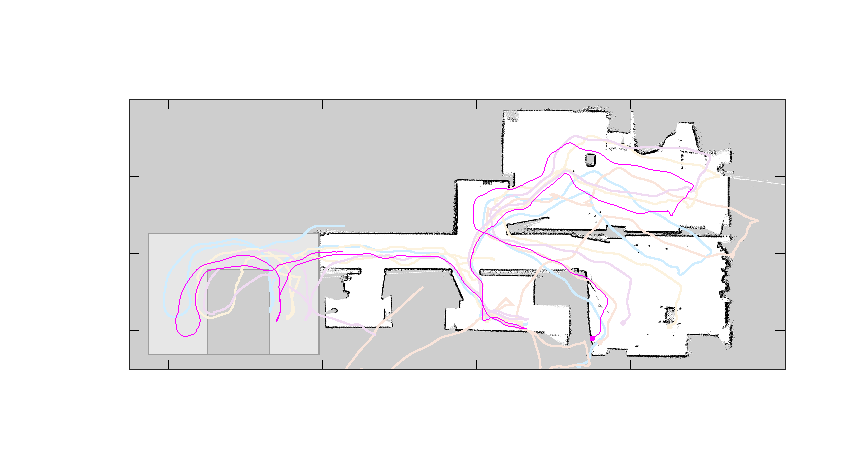
\includegraphics[scale=0.67]{./figures/slides/ch7/odom/real/odom_test_ag10/odom_test_10}}%
    \gplfronttext
  \end{picture}%
\endgroup

  \end{minipage}
\end{figure}


\note{\footnotesize
Εδώ τώρα θέλω να σας δείξω πώς μεταφράζονται στην πράξη αυτά τα σφάλματα. Εδώ
βλέπουμε με διαφορετικά χρώματα την εκτίμηση της τροχίας ενός πραγματικού
αισθητήρα YDLIDAR από τους αλγορίθμους της πειραματικής διαδικασίας που τρέχουν
σε πραγματικό χρόνο στα αριστερά, και στα δεξιά τον fsm. Εδώ παρατηρούμε πως το
σφάλμα θέσης κάθε μεθόδου αυξάνει στις μεταβάσεις του αισθητήρα απο δωμάτιο
σε δωμάτιο ακριβώς λόγω των καινούριων περιοχών που μπαίνουν στο πεδίο όρασης
του αισθητήρα, οι οποίες δεν υπάρχουν στις προηγούμενες σαρώσεις, και οι
οποίες συνεπώς παράγουν κενές αντιστοιχίες ανάμεσα σε δύο διαδοχικές
σαρώσεις.  Ο αισθητήρας περνάει από πέντε τέτοια σημεία για συνολικά εννιά
φορές. Η εκτιμώμενη απόσταση που διένυσε ο αισθητήρας είναι 43 μέτρα. Οι
εκτιμώμενες τροχιές του έχουν ευθυγραμμισθεί με βάση αυτά τα σημεία επειδή
δεν έχουμε πρόσβαση στην πραγματική τροχιά του αισθητήρα, και από ότι βλέπετε
ο fsm έχει τη μικρότερη απόκλιση μέσα στο χρόνο σε σχέση με τις μεθόδους της
τρέχουσας βιβλιγραφίας.
}

\end{frame}
